\documentclass[12pt]{article}
\usepackage[margin=0.7in]{geometry}
\usepackage{setspace}
\usepackage{graphicx}
\usepackage{hyperref}
\usepackage{amsmath}
\usepackage{amssymb}
\usepackage{listings}
\usepackage{float}
\usepackage{subfig}
\usepackage[]{algorithm2e}
\RestyleAlgo{boxruled}
\usepackage{rotating}

\newcommand{\deriv}[3][]{% \deriv[<order>]{<func>}{<var>}
  \ensuremath{\frac{\partial^{#1} {#2}}{\partial {#3}^{#1}}}}
\newcommand{\atconstant}[2]{\ensuremath{\left( #1 \right)_{#2}}}
\begin{document}
\title{PHYS 849: Assignment 2}
\author{Jake Bauer}
\date{\today}
\maketitle

\section*{Problem 1}
The Poisson distribution is given as,
\begin{equation}
\mathbb{P}(x = k \,| \,\mu) = \frac{e^{-\mu} \mu^k}{k!}.
\end{equation}
The characteristic function of the distribution is given by its discrete Fourier transform (DFT),
\begin{eqnarray}
\phi(\omega) &=& \mathcal{F}\{\mathbb{P}(x = k \,| \,\mu) \}\\
&=& e^{-\mu} \sum_{k=0}^{N} \frac{ \mu^k}{k!} \times e^{ i \omega k}\\
&=&  e^{-\mu} \sum_{k=0}^{N} \frac{\left( \mu e^{i \omega}\right)^k}{k!}.
\end{eqnarray}
We point out that the sum is clearly just the definition of a Taylor expansion for a function whose derivatives are,
\begin{eqnarray}
\frac{\text{d}^k f(\omega)}{\text{d} \omega^k} &=& \mu^k e^{ i k \omega}.
\end{eqnarray}
The function which satisfies this is,
\begin{equation}
f(\omega) = \exp\left[ {\mu} e^{ i\omega}\right],
\end{equation}
which implies that the characteristic function is,
\begin{equation}
\phi(\omega) = \exp\left[ \mu \left( e^{i \omega}- 1\right)\right].
\end{equation}
Evaluating this function at zero gives the normalization,
\begin{eqnarray}
\phi(0) &=& \exp\left[ \mu \left( e^{i \times 0} - 1\right)\right]\\
&=& 1,
\end{eqnarray}
which is exactly as expected. The first algebraic moment (mean) is,
\begin{eqnarray}
\left. \frac{\text{d} \phi}{\text{d} \omega} \right \vert_{\omega = 0} &=& \exp\left[ \mu \left( e^{i \times 0 } - 1\right)\right] \times \left(\mu e^{ i \times 0 }  \right) \times i\\
&=& 1 \times \mu \times i\\
&=& i \mu.
\end{eqnarray}
Then it follows that $\mathbb{E}(X) = \mu$ from $\phi^{(n)}(0) = i^n \mathbb{E}(X^n)$. We perform the same analysis for the second algebraic moment,
\begin{eqnarray}
\left. \frac{\text{d}^2 \phi}{\text{d} \omega^2} \right \vert_{\omega = 0} &=& \left(\frac{\text{d}}{\text{d} \omega} \frac{\text{d} \phi}{\text{d} \omega}\right)_{\omega = 0 }\\
&=&\left(\frac{\text{d}}{\text{d} \omega} \exp\left[ \mu \left( e^{i \omega } - 1\right)\right] \times \left(\mu e^{ i \omega }  \right) \times i\right)_{\omega = 0}\\
&=& \left( \exp\left[ \mu \left( e^{i \omega } - 1\right)\right] \times \left(\mu e^{ i \omega }  \right)^2 \times i^2 + \exp\left[ \mu \left( e^{i \omega } - 1\right)\right] \times i^2 \mu e^{i \omega}\right)_{\omega=0}\\
&=& 1 \times \mu^2 \times i^2 + 1 \times i^2 \times \mu\\
&=& i^2(\mu^2 + \mu),
\end{eqnarray}
which gives $\mathbb{E}(X^2) = \mu^2 + \mu$.  The variance is then $\sigma^2 =  \mu^2 - \mu^2 + \mu = \mu$. The standard deviation is then $\sigma = \sqrt{\mu}$.

\section*{Problem 2}
\subsection*{(a)}
The first algebraic moment of the uniform distribution is,
\begin{eqnarray}
\mathbb{E}(X) = \int_0^1 x \text{d} x\\
&=& \frac{1}{2}.
\end{eqnarray}
The second algebraic moment is,
\begin{eqnarray}
\mathbb{E}(X^2) = \int_0^1 x^2 \text{d}x\\
&=& \frac{1}{3}.
\end{eqnarray}
The variance is then $\sigma^2 = \frac{1}{3} - \frac{1}{4} =  \frac{1}{12}$.  The standard deviation is then $\frac{1}{\sqrt{12}}$.

\subsection*{(b)}
Figure \ref{fig:uniform} shows the requested information.

\subsection*{(c)-(f)}

Figure \ref{fig:clt} shows the requested information for the $N$-point sum distribution.  This can be presented differently by considering the distribution of $N$-point averages. Figure \ref{fig:clt_average} shows the distribution of these averages.  We note from the left panel that all means are at 0.5, as expected, with variances decreasing with the number of sample points.  The right panel shows this same behavior in log space to highlight how the Gaussian limit is better achieved with large $N$.  

\subsection*{(g)}

To conclude, we have demonstrated that taking $N$-tuple sample sums from an initially uniform distribution results in the sums being distributed according to the central limit theorem.  That is, the mean of the $N$-tuple sum is approximately $N \mu$, where $\mu$ is the mean of the distribution of the tuple elements, $\mathbb{E}(U(0,1)) = 0.5$. We have also shown that the variances sum linearly, i.e., the standard deviations add in quadrature.  That is, we expect the standard deviation for an $N$-tuple sum to be $\sigma_p^2 = N \sigma^2 = N\times \frac{1}{12}$.  As $N$ increases, absolute differences between the normalized bin heights and the expected Gaussian distributions decrease, and the sample statistics approach the expected values.  Considering the distribution of $N$-point averages, we better see this convergence property.  We expect the sample variance,
\begin{equation}
\text{Var}[\mathbb{E}(S \subset X)] = \frac{1}{\vert S \vert}\sum_{i=0}^{\vert S \vert} (s - \mu)^2,
\end{equation}
to decrease as $1 / N$.  Here, $s$ is the $N$-point average sample, and $\mu$ is its expected value of 0.5. These definitions imply our expectation because $\vert S \vert = 10^4$, and $s = \frac{1}{N}\sum_i x_i$. In fact, we see this is roughly true in Table \ref{tab:convergence}.  Consider the difference between 100 and 1000.  In theory, we expect,
\begin{eqnarray}
\sigma_{1000} &=& \sqrt{\frac{100}{1000}} \times \sigma_{100}\\
0.0287,
\end{eqnarray}
or roughly the 0.0281 that is actually calculated from the sample.
\begin{table}
\centering
\caption{Mean and standard deviation for the distribution of $N$-point averages.} \label{tab:convergence}
\begin{tabular}{|l|l|l|}
\hline
$N$ & $\mu$ & $\sigma$\\
\hline
2 & 0.50099 & 0.28798\\
10 & 0.49952 & 0.20281\\
100 & 0.50189 & 0.09142\\
1000 & 0.50057& 0.02807\\
\hline
\end{tabular}
\end{table}
\newpage
\begin{figure}
\centering
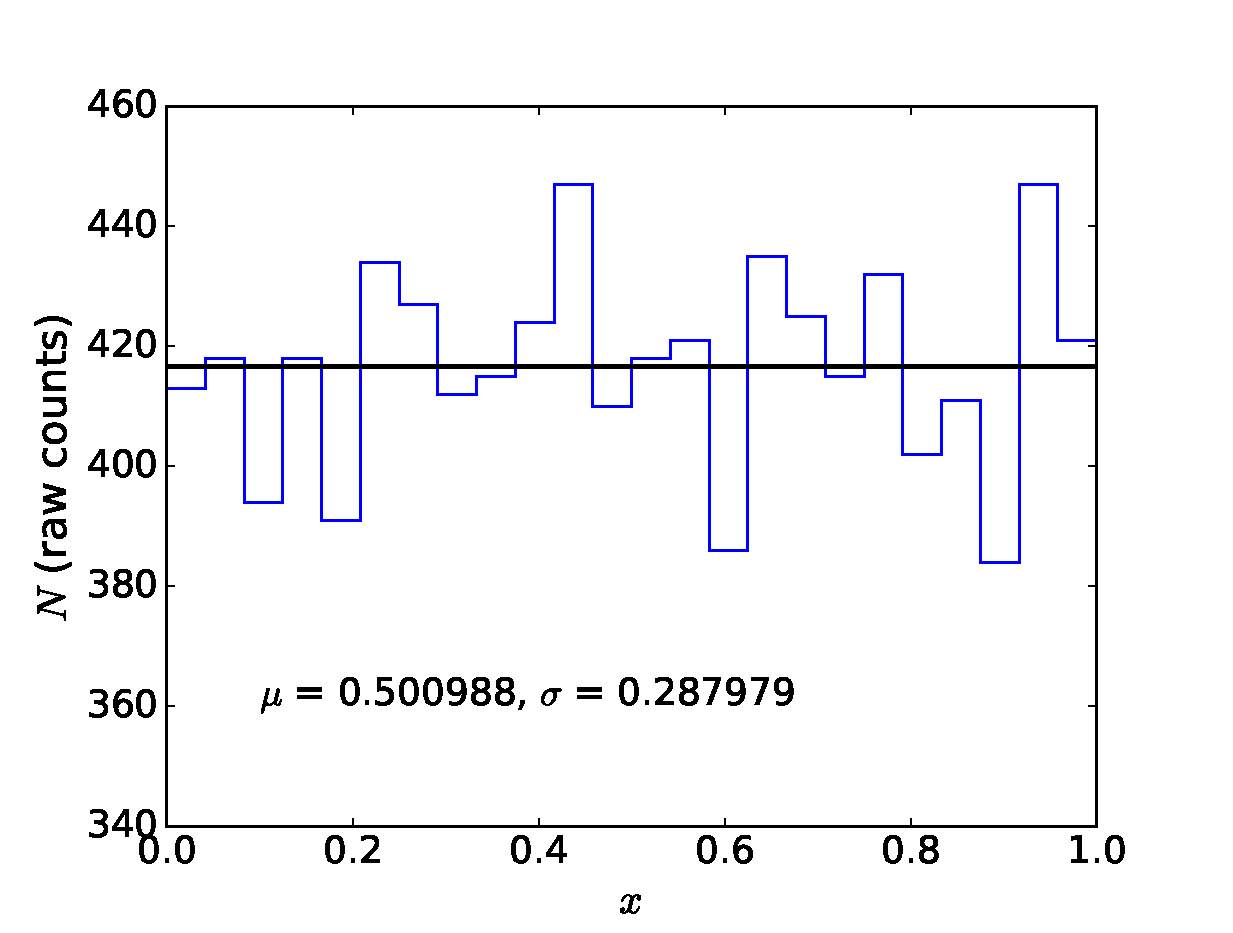
\includegraphics[width=0.5\textwidth]{uniform_sample.eps}
\caption{A uniform sample on $[0,1]$. The solid black line shows the expected continuum limit.} \label{fig:uniform}
\end{figure}

\begin{figure}
\centering
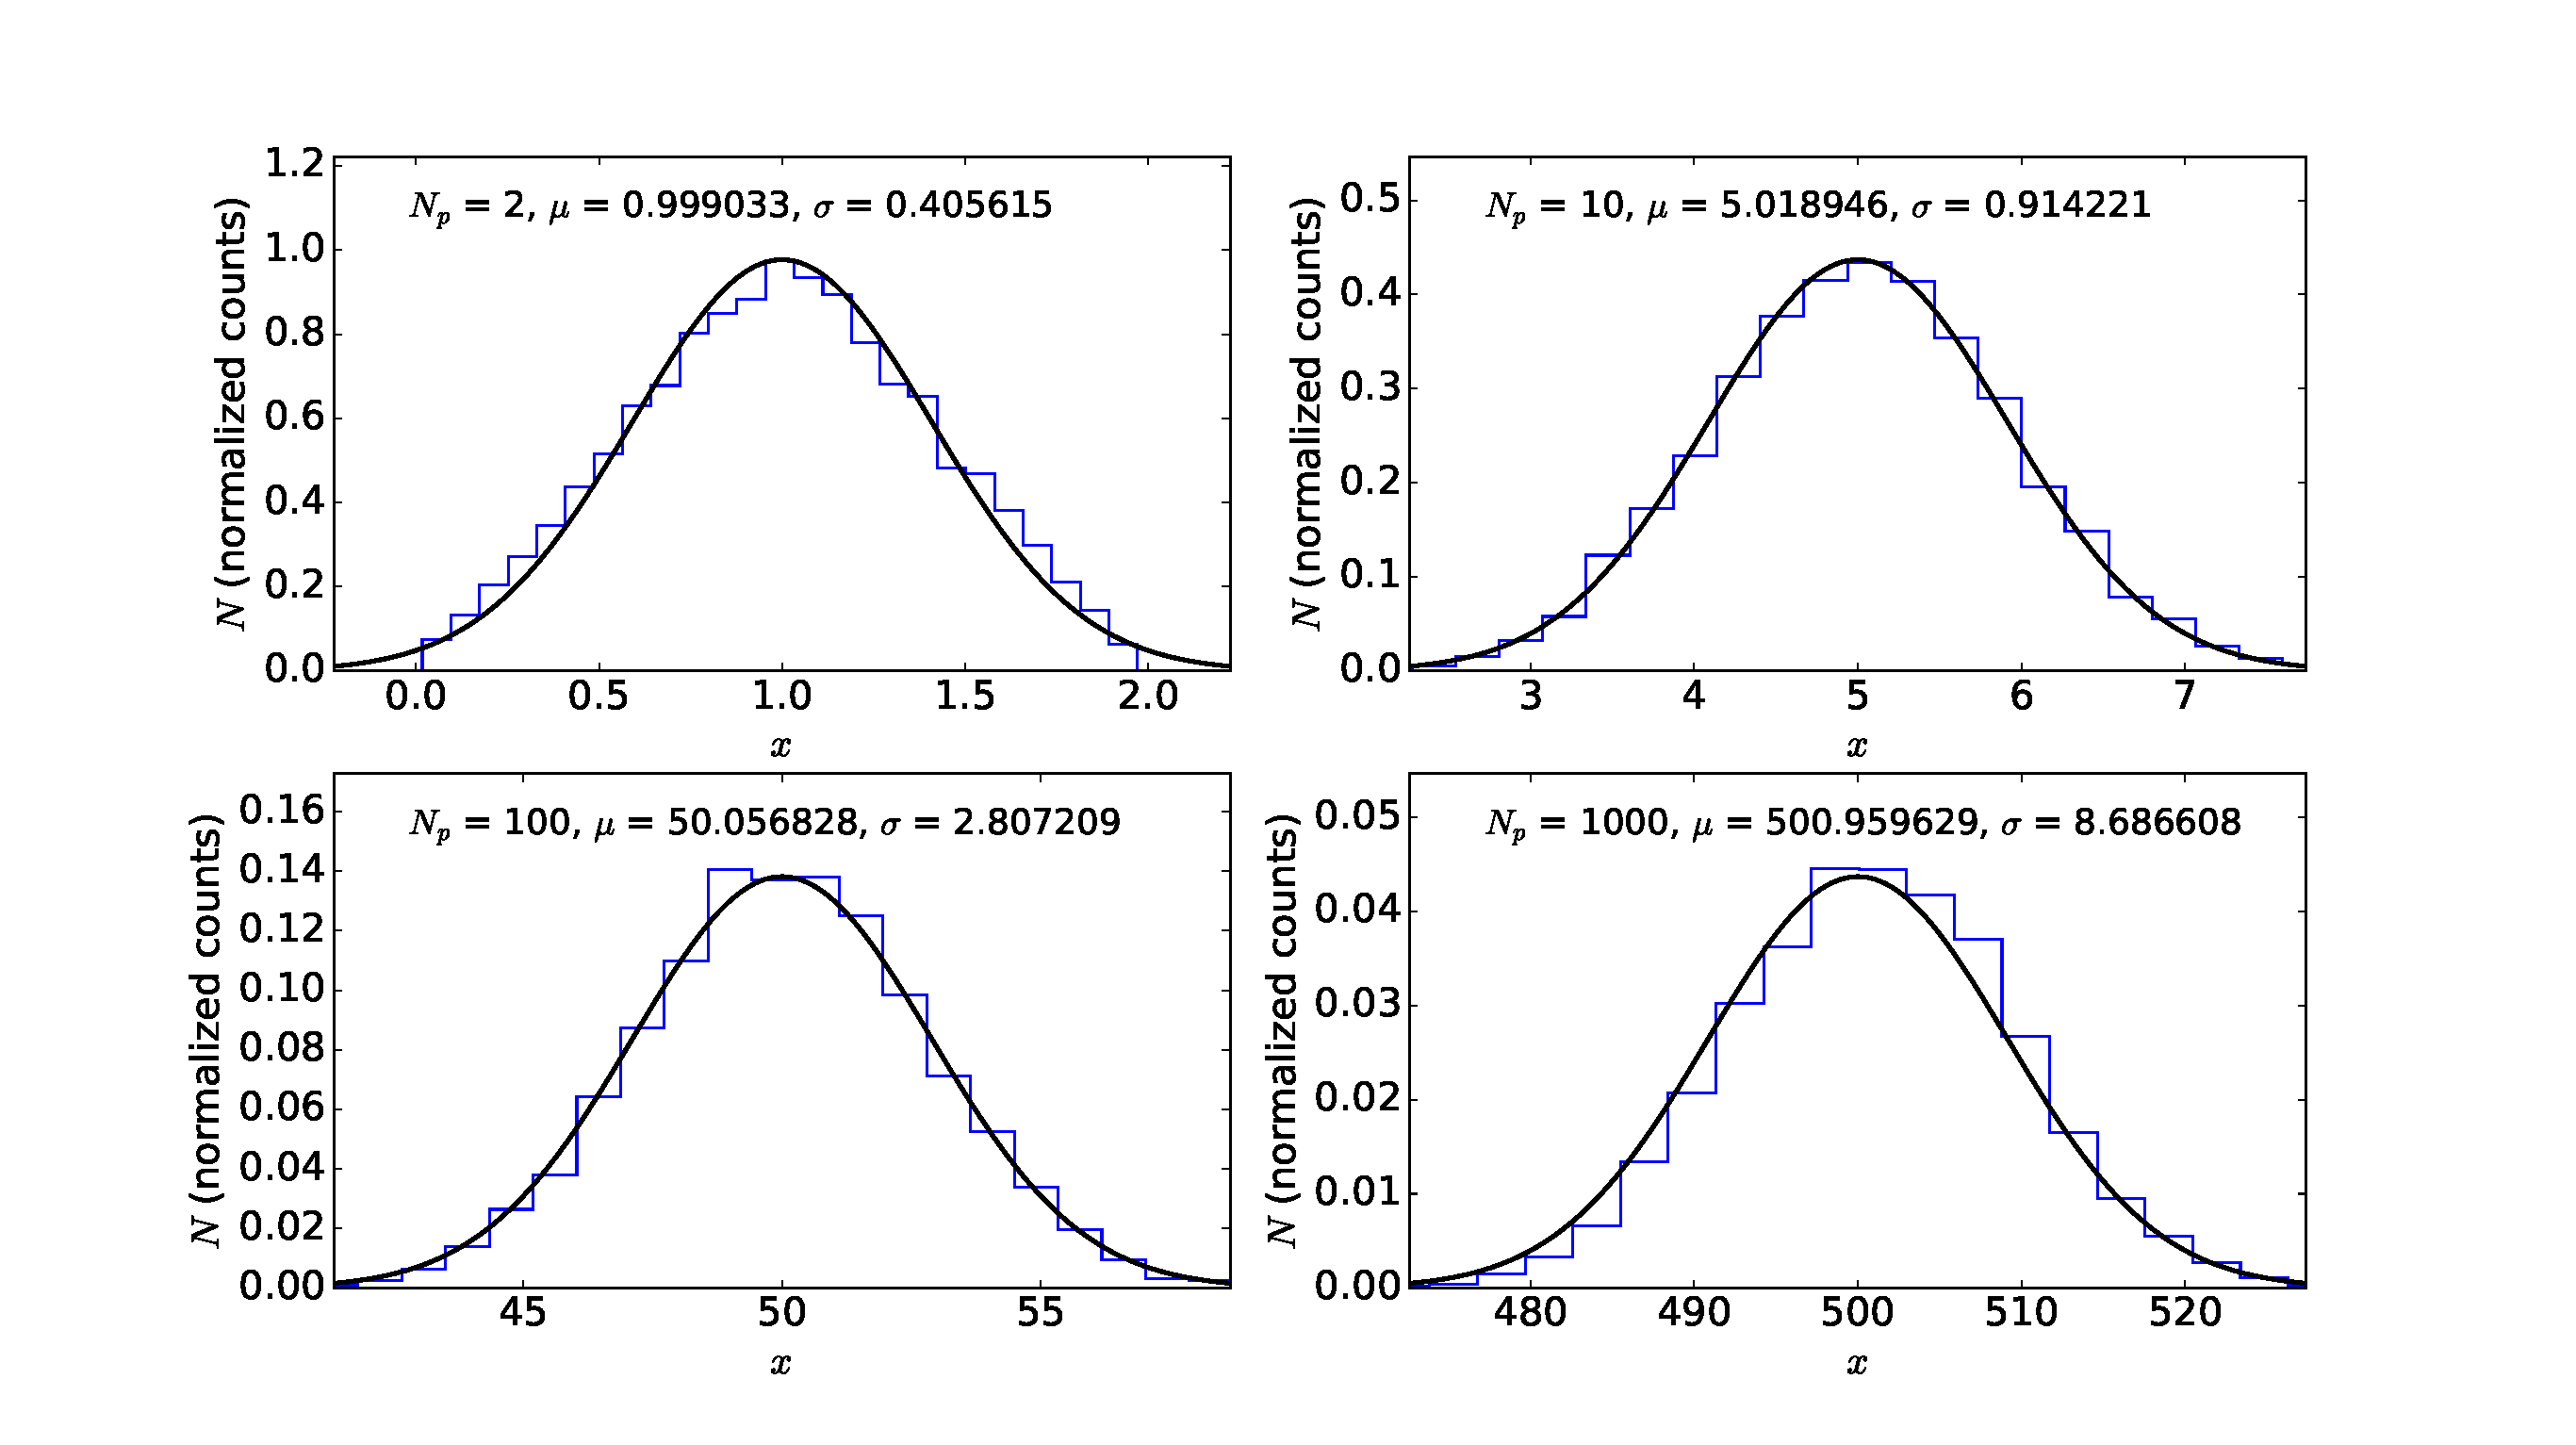
\includegraphics[width=1.1\textwidth]{clt.eps}
\caption{Four panels of $N$-wise joint sum distributions.  The panels are annotated with the number of sum elements, $N_p$, and the CLT expected Gaussian parameters.  The black line then shows the CLT predicted Gaussian for these joint sums.} \label{fig:clt}
\end{figure}


\begin{figure}
\centering
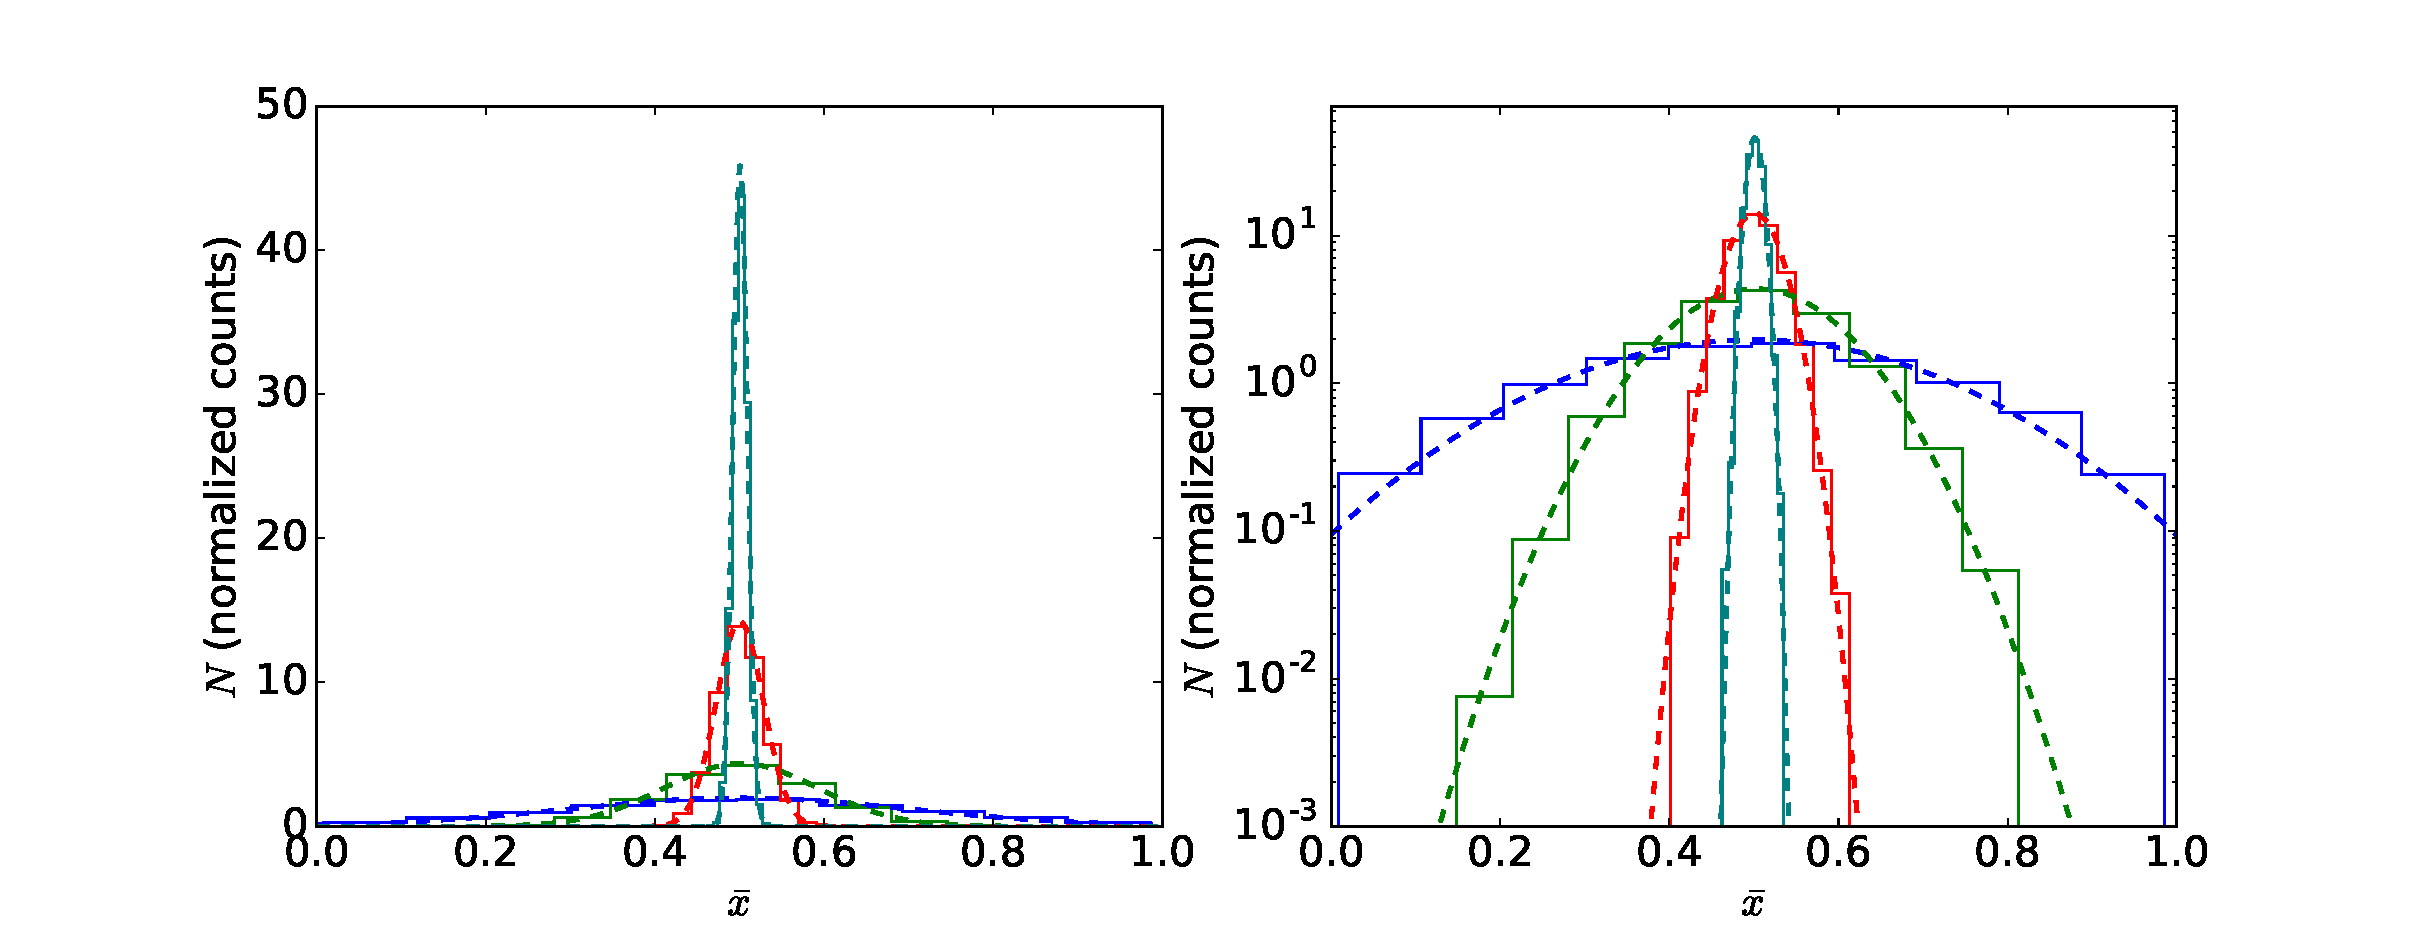
\includegraphics[width=1.\textwidth]{clt_average.eps}
\caption{The left panel shows the distribution of random $N$-point averages (histograms) with the expected distribution overlaid (dashed).  The right panel shows the same on a log scale.  The color scheme is $N=2$ (blue), $N=10$ (green), $N=100$ (red), and $N=1000$ (teal).} \label{fig:clt_average}
\end{figure}

\end{document}


%\subsection*{(c)-(f)}
